\newpage
\section{Math101 exercises}
\begin{enumerate}
	
	\item Let $f(x)=3x^2+2x+1$. Determine $f(-1)$ and $f(2)$.
	
	\item \label{it:5} The circle given by the equation $x^{2} +(y-1)^{2}=1$ is sketched in Figure~\ref{fig:5}.
	\begin{itemize}
		\item Does there exist a function $f\colon [-1,1]\to [0,2]$ such that the graph of $f$ is the circle in Figure~\ref{fig:5}?
		\item Determine a function $f_+\colon [-1,1]\to [1,2]$ such that the graph of $f_+$ is the upper semi circle in Figure~\ref{fig:5}.
		\item Determine a function $f_-\colon [-1,1]\to [0,1]$ such that the graph of $f_-$ is the lower semi circle in Figure~~\ref{fig:5}.
	\end{itemize}	
	\begin{figure}
		\centering
		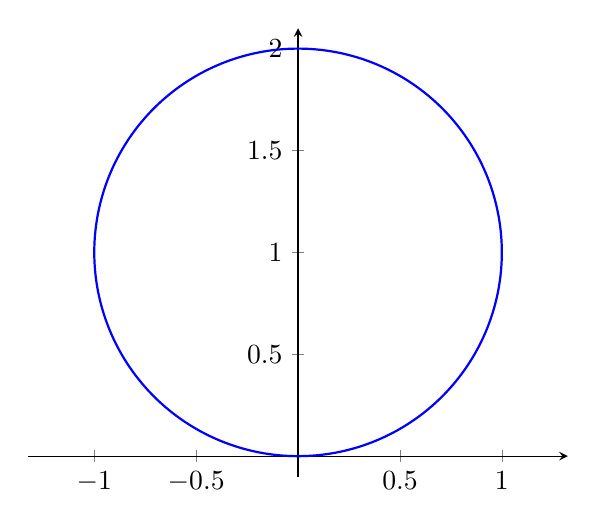
\begin{tikzpicture}
		\begin{axis}[xmin=-1.1,xmax=1.1,ymin=-0.1,ymax=2.1,axis x line=center,
		axis y line=center,axis equal, restrict y to domain=-2:2]
		\addplot[thick,blue,domain=0:2*pi,samples =800] ({cos(deg(x))},{1+sin(deg(x))});
		\end{axis}
		\end{tikzpicture}
		\caption{Exercise~\ref{it:5}.}
		\label{fig:5}
	\end{figure}

	
	\item Let $f(x)=3x-2$ and $g(x)=\frac{1}{3}x+\frac{2}{3}$. Determine the function $f\circ g$.
	
	
		\item Find the domain of the functions:
	\begin{align*}
	f(x)=\frac{1}{x+1},&& g(x)=\frac{1}{1-x^2},&& h(x)=\sqrt{2x-3}.
	\end{align*}
	
	
	\item  Let $f,g$ be given by $f(x)=\sqrt{x}$ and $g(x)=1/(1+x)$ on the domain $(0,\infty)$. Calculate $(f\circ g)(1)$ and $(g\circ f)(1)$. Is $f\circ g=g\circ f$?
	
	\item Determine the intersection between $f(x)=3x+1$ and $g(x)=-x+2$.	
	
	\item Let $f(x)=1$ and $g(x)=2x+3$. Determine $f\circ g$ and $g\circ f$.
	
	
	\item What is the largest possible domain of definition for the functions:
	\begin{align*}
	f(x)=\frac{1}{(1+x^2)^\frac{1}{2}},&& g(x)=\frac{2}{x^2-4x+3},&& h(x)=\sqrt{-x^2+2x}.
	\end{align*}
	
	
	\item Determine functions $f$ and $g$ such that $(f\circ g)(x)=e^{2x^2-1}$.
	
	\item Determine all intersection points between $f(x)=x^2+4x+4$ and $g(x)=2x+3$.
	
	\item Determine functions $f$, $g$ and $h$ such that $(f\circ g\circ h)(x)=\sin^2(3x)$. (Hint: $ \sin^2(x)=(\sin(x))^2 $.)
	
	\item Let $f(x)=3(\frac{1}{x-2})^2$, $g(x)=\frac{1}{x}$ and $h(x)=\sqrt{x}+2$ be functions defined on the domain $]2,\infty[$. Determine
	\begin{align*}
	f(g(x)),&& f(h(x)),&& h(g(x)),&& h(f(x)),&&g(f(h(x))).
	\end{align*} 
	
		\item\label{it:fun3} Is the curve in Figure~\ref{fig:fun3} the graph of a function?
	\begin{figure}
		\centering
		\begin{tikzpicture}
		\begin{axis}[xmin=-5,xmax=5,ymin=-5,ymax=5,axis x line=center,
		axis y line=center, restrict y to domain =-5:5]
		\addplot[data cs=polar, thick,blue,samples=200, domain= 0:180] ({x}, {3*sin(x)*cos(x)/(sin(x)^3+cos(x)^3)});
		\end{axis}
		\end{tikzpicture}
		\caption{Exercise~\ref{it:fun3}.}
		\label{fig:fun3}
	\end{figure}

	\item Sketch the graph of a function which
	\begin{enumerate}
	\item has domain $[-1,1]$,
	\item intersects the points $(-1,0)$ and $(1,1)$,
	\item intersects the $y$-axis at $-1$,
	\end{enumerate}
	
\end{enumerate}